%%%%%%%%%%%%%%%%%%%%%%%%%%%%%%%%%%%%%%%%%
% Journal Article
% LaTeX Template
% Version 1.3 (9/9/13)
%
% This template has been downloaded from:
% http://www.LaTeXTemplates.com
%
% Original author:
% Frits Wenneker (http://www.howtotex.com)
%
% License:
% CC BY-NC-SA 3.0 (http://creativecommons.org/licenses/by-nc-sa/3.0/)
%
%%%%%%%%%%%%%%%%%%%%%%%%%%%%%%%%%%%%%%%%%

%----------------------------------------------------------------------------------------
%	PACKAGES AND OTHER DOCUMENT CONFIGURATIONS
%----------------------------------------------------------------------------------------

\documentclass[twoside]{article}

\usepackage{lipsum} % Package to generate dummy text throughout this template
\usepackage[french]{babel}

\usepackage[utf8]{inputenc}

\usepackage[sc]{mathpazo} % Use the Palatino font
\usepackage[T1]{fontenc} % Use 8-bit encoding that has 256 glyphs
\linespread{1.05} % Line spacing - Palatino needs more space between lines
\usepackage{microtype} % Slightly tweak font spacing for aesthetics

\usepackage[hmarginratio=1:1,top=32mm,columnsep=20pt]{geometry} % Document margins
\usepackage{multicol} % Used for the two-column layout of the document
\usepackage[hang, small,labelfont=bf,up,textfont=it,up]{caption} % Custom captions under/above floats in tables or figures
\usepackage{booktabs} % Horizontal rules in tables
\usepackage{float} % Required for tables and figures in the multi-column environment - they need to be placed in specific locations with the [H] (e.g. \begin{table}[H])
\usepackage{hyperref} % For hyperlinks in the PDF

%\usepackage{lettrine} % The lettrine is the first enlarged letter at the beginning of the text
\usepackage{paralist} % Used for the compactitem environment which makes bullet points with less space between them

\usepackage{abstract} % Allows abstract customization
\renewcommand{\abstractnamefont}{\normalfont\bfseries}
\renewcommand{\abstractname}{Résumé} % Set the "Abstract" text to bold
\renewcommand{\abstracttextfont}{\normalfont\small\itshape} % Set the abstract itself to small italic text

\usepackage{titlesec} % Allows customization of titles
\renewcommand\thesection{\Roman{section}} % Roman numerals for the sections
\renewcommand\thesubsection{\arabic{subsection}.\arabic{subsection}} % Roman numerals for subsections
\titleformat{\section}[block]{\bfseries\large\scshape\centering}{\thesection.}{1em}{} % Change the look of the section titles
\titleformat{\subsection}[block]{\bfseries\large}{\thesubsection.}{1em}{} % Change the look of the section titles

\usepackage{fancyhdr} % Headers and footers
\pagestyle{fancy} % All pages have headers and footers
\fancyhead{} % Blank out the default header
\fancyfoot{} % Blank out the default footer
\renewcommand{\headrulewidth}{0pt} %pour enlever la ligne du header
%\fancyhead[C]{titre, date, noms...	} % Custom header text
\fancyfoot[RO,LE]{\thepage} % Custom footer text


%agrandissement de la zone de texte
\addtolength{\oddsidemargin}{-1cm}
\addtolength{\evensidemargin}{-1cm}
\addtolength{\textwidth}{2cm}

%pour les maths
\usepackage{amsmath}
\usepackage{amsfonts}

%pour les images
\usepackage{graphicx}
\usepackage{caption}

\renewcommand\arraystretch{1.4}

%----------------------------------------------------------------------------------------
%	TITLE SECTION
%----------------------------------------------------------------------------------------

\title{\vspace{-15mm}\fontsize{24pt}{10pt}\selectfont\textbf{Imagerie ultrasonore multi-éléments pour la caractérisation de défauts de soudure}} % Article title

\author{
\large
{Alice \textsc{Dinsenmeyer} \& Thomas \textsc{Lechat}}\\[2mm] % Your name %\thanks{}
%\normalsize University of California \\ % Your institution
%\normalsize \href{mailto:john@smith.com}{john@smith.com} % Your email address
\vspace{-5mm}
}
\date{}

%----------------------------------------------------------------------------------------

\begin{document}

\maketitle % Insert title

\thispagestyle{fancy} % All pages have headers and footers

%----------------------------------------------------------------------------------------
%	ABSTRACT
%----------------------------------------------------------------------------------------

\begin{abstract}
\noindent L'imagerie multi-éléments repose sur le même principe que les antennes à commande de phase : le transducteur utilisé est constitué de plusieurs éléments piézoélectriques pouvant émettre et recevoir des signaux haute fréquence.
 Afin de comprendre son utilisation en contrôle de pièces industrielles, trois défauts de soudure sont imagés à l'aide d'un boîtier Sofranel. La qualité de leur représentation dépend surtout de la précision sur la position des capteurs lors de la mesure et des nombreux réglages effectués en amont. 

\end{abstract}

%----------------------------------------------------------------------------------------
%	ARTICLE CONTENTS
%----------------------------------------------------------------------------------------

\begin{multicols}{2} % Two-column layout throughout the main article text

\section{Introduction}

Connue pour son usage répandu en médecine, l'imagerie multi-éléments par ultrasons est également largement employées dans le secteur de l'industrie. En effet, elle peut fournir rapidement des images précises, ce qui est adapté à de l'imagerie de soudure, de collage, de fissure, du contrôle d'épaisseur, etc. 

Ce rapport revient sur cette méthode, appliquée à de l'imagerie d'une soudure en V sur plaque d'acier de 8 mm d'épaisseur.
%------------------------------------------------

\section{Principe de l'imagerie multi-éléments}

Le transducteur utilisé pour l'imagerie multi-éléments est une barrette composée de plusieurs éléments piézoélectriques. Disposée en ligne ou en matrice, ils peuvent être excité avec suivant une loi de retard permettant de focaliser et de diriger le front d'onde. La figure~\ref{multielements} montre qu'une loi de retard linéaire (à gauche) permet de générer et de diriger un front d'onde plan, tandis que d'autres lois permettent, par exemple de focaliser l'énergie et de déplacer ce point de focalisation (image de droite).

Ce même transducteur est utilisé pour la réception du signal réfléchi.

\begin{figure}[H]
	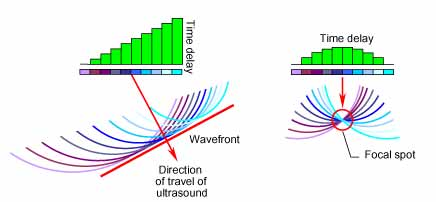
\includegraphics[scale=0.5]{images/principe.jpg}
		\caption{Lois de retard appliquées aux éléments pour générer un front d'onde plan (à gauche) ou focaliser en un point (image : http://www.twi-global.com)\label{multielements}}
\end{figure}

Cette méthode présente donc l'intérêt de pouvoir effectuer des balayages rapides, fournissant une image 2D sans déplacement du transducteur. Elle est donc adaptée à un usage industriel, pour des pièces de géométrie complexe ou partiellement accessibles. De plus, la focalisation dans la matière permet d'obtenir un bon rapport signal sur bruit.

Ses inconvénients sont le prix du matériel, de part la complexité de sa fabrication, et le niveau technique que requiert son utilisation. 

%------------------------------------------------

\section{Mesures}

\subsection{Géométrie de la soudure}

La soudure caractérisée ici comporte trois types de défauts connus : une fissure, un défaut de porosité et défaut de fusion. La figure~\ref{soudure} montre leur placement sur la soudure (coupe transversale) et le tableau~\ref{position} indique leur position sur la longueur.

\begin{figure}[H]
	\centering
	
\includegraphics[scale=0.9]{images/soudure.png}
	\caption{\label{soudure}Vue en coupe transversale des défauts de la soudure.}
\end{figure}

\begin{table}[H]
	\centering
	\begin{tabular}{c | c | c}
		N\textsuperscript{o} du défaut & Type de défaut & Position (mm) \\\hline
		\textcircled{\footnotesize 1} & Fissure & 40 \\ \hline
		\textcircled{\footnotesize 2} & Porosité & 117 \\ \hline
		\textcircled{\footnotesize 3} & Manque de fusion & 240 \\ 
	\end{tabular}	
	\caption{\label{position}Tableau répertoriant les défauts et leur position le long de la soudure, par rapport au bord de la plaque.}
\end{table}

\subsection{Procédé expérimental}

Le contrôle du transducteur ainsi que les traitement du signal et de l'image sont effectués par le boîtier \textit{veo 16:64} de \textit{Sonatest}. L'utilisateur a seulement besoin de renseigner la géométrie de la soudure, le matériel utilisé et le type de focalisation. Elle est choisie de manière a balayer le plus largement possible la soudure.

Le transducteur utilisé comporte 64 éléments\footnote{Sonatest, X3-PE-5.OM64EO.6P}. Sa fréquence centrale est 5 MHz. Un sabot, en Plexiglas, sert a générer des ondes transversales (T). La longueur d'onde de ces ondes étant plus faible que celle des ondes longitudinales (L), elles permettent une meilleure précision.

L'angle du sabot est donc choisi de façon à ce l'angle d'incidence soit situé au-delà de l'angle critique pour les ondes L et en-deçà de l'angle critique pour les ondes T dans l'acier.
Pour cela, il est nécessaire de connaître la vitesse des ondes dans chaque matériau. La vitesse des ondes L dans le sabot est donnée par le fabricant. La vitesse des ondes T et L dans l'acier est estimée à partir du module d'Young ($E\approx 200$ GPa) et du coefficient de Poisson ($\nu \approx 0.3$)du matériau. La loi de Snell-Descartes permet ensuite de connaître les angles critiques (angle d'incidence pour lequel l'angle de réfraction est de $90^{\circ}$) pour les différentes ondes. Toutes ces valeurs sont présentées dans le tableau ci-dessous.

\begin{center}
	\begin{tabular}{c| c ||c |c }
		& Plexiglas & \multicolumn{2}{c}{Acier} \\ \hline
		& Ondes L & Ondes L & Ondes T \\ \hline
		Vitesse (m/s) & $V_{plexi}^{L}= 2337$ & $V_{acier}^{L}= 5947$ & $V_{acier}^{T}= 3181$ \\ \hline
		Angle critique && $23^{\circ}$ &  $47^{\circ}$\\
	\end{tabular}
\end{center}

Pour générer des ondes T dans l'acier, le sabot\footnote{Sonatest, SB57-N455} choisi est donc incliné à $30^{\circ}$. À 5 MHz, la longueur de ces ondes est d'environ 0.6 mm dans l'acier, ce qui est de l'ordre de grandeur des défauts à trouver.



\subsection{Imagerie des défauts}

Les S-scans réalisés au niveau des défauts sont présentés en figure~\ref{resultat}. 


\begin{figure}[H]
	\centering
	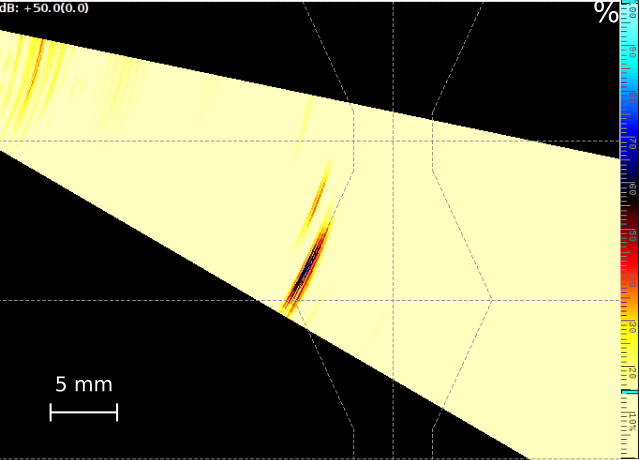
\includegraphics[width=5cm]{images/def1.png}\\
	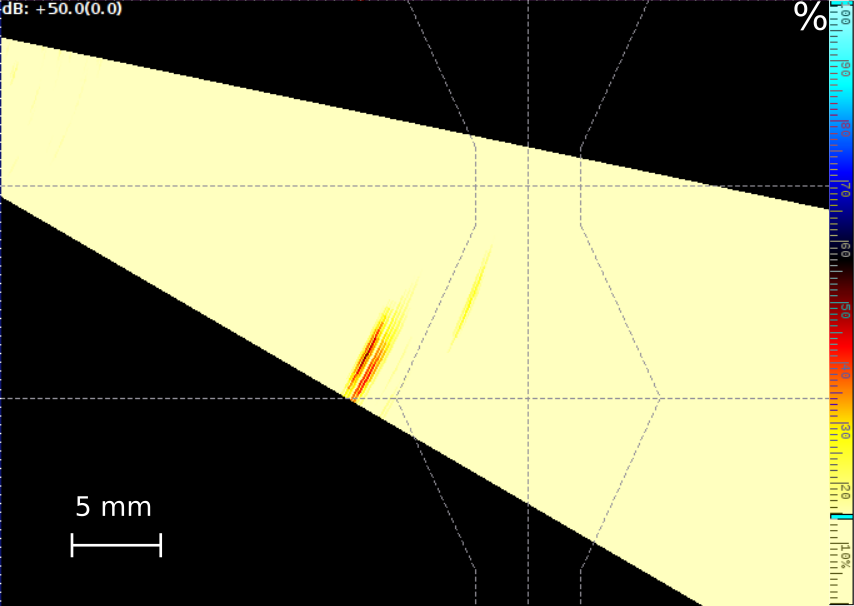
\includegraphics[width=5cm]{images/def2.png}\\
	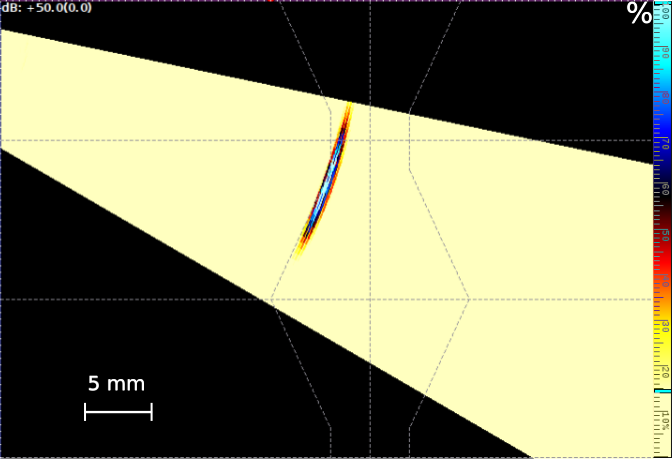
\includegraphics[width=5cm]{images/def3.png}\\
	\caption{\label{resultat} Résultat des mesures au niveau des défauts \textcircled{\footnotesize 1}, \textcircled{\footnotesize 2} et \textcircled{\footnotesize 3} (de haut en bas).}
\end{figure}

Les deux premiers scans donne une position erronée du défaut. Le premier défaut devrait être situé à la racine de la soudure et le second au centre. Ce décalage provient d'une imprécision sur la position du transducteur sur la plaque. Manipulé à la main, il a pu ne pas rester tout à fait d'équerre et sa distance à la soudure a pu changer également légèrement. Il apparaît donc que l'image est très sensible à la position du transducteur et qu'un guide précis aurait du être utilisé pour réaliser les scans.\\

Il est difficile d'évaluer sans expérience le type de défaut par simple observation des images. La porosité apparaît d'amplitude plus faible et sous forme de réflexions multiples, mais les deux autres défauts se ressemblent beaucoup.\\

Enfin, il est à noter que ces images sont le résultats d'un paramétrage optimisé de la focalisation pour observer au mieux les défauts, dont la position étaient connues. Il s'avère qu'un mauvais choix de focalisation peut compromettre la qualité d'un contrôle, car c'est un paramètre sensible qui peut rendre un défaut invisible.
%------------------------------------------------

\section{Conclusion}

Ces trois exemples de défauts couramment rencontrés en contrôle de soudures montrent que l'imagerie multi-éléments peut donner des représentations précises d'inhomogénéités dans un matériau isotrope. \\
Les boîtiers commercialisés à cet effet ne nécessitent pas de connaissance en traitement du signal, mais exige de l'attention lors des réglage et de la précision lors de la mesure.


%----------------------------------------------------------------------------------------
%	REFERENCE LIST
%----------------------------------------------------------------------------------------

%\begin{thebibliography}{99} % Bibliography - this is intentionally simple in this template
%
%\bibitem[Figueredo and Wolf, 2009]{Figueredo:2009dg}
%Figueredo, A.~J. and Wolf, P. S.~A. (2009).
%\newblock Assortative pairing and life history strategy - a cross-cultural
%  study.
%\newblock {\em Human Nature}, 20:317--330.
% 
%\end{thebibliography}

%----------------------------------------------------------------------------------------

\end{multicols}

\end{document}
